
\begin{document}

% @see : https://coopmaths.fr/alea?uuid=01873&id=6C20&n=2&d=10&s=3&s2=3&s3=4&alea=hgRP234567891011121314&cd=1&cols=1
\begin{EXO}{}{6C20}
Poser et effectuer les calculs suivants.

\begin{enumerate}[itemsep=2em]
	\item $131+69{,}23$
	\item $505-499{,}7$
\end{enumerate}
\end{EXO}

% @see : https://coopmaths.fr/alea?uuid=52939&id=6C30&n=1&d=10&s=false&s2=3&alea=2Cpi234567891011121314&cd=1&cols=1
\begin{EXO}{}{6C30}
Poser et effectuer les calculs suivants.

 $97{,}4\times9{,}8$
\end{EXO}

% @see : https://coopmaths.fr/alea?uuid=29c3b&id=6G53&n=1&d=10&alea=VP3Q234567891011121314&cd=1&cols=1
\begin{EXO}{}{6G53}


 Mesurer la distance entre le point $T$ et la droite ($d$).\\\begin{tikzpicture}[baseline]

    \tikzset{
      point/.style={
        thick,
        draw,
        cross out,
        inner sep=0pt,
        minimum width=5pt,
        minimum height=5pt,
      },
    }
    \clip (-5,-4) rectangle (5,5);
    	\draw[color ={{black}},line width = 0.625,opacity = 0.8] (-1.0625,3.0625)--(-0.9375,2.9375);\draw[color ={{black}},line width = 0.625,opacity = 0.8] (-1.0625,2.9375)--(-0.9375,3.0625);
	\draw [color={black}] (-1,3.5) node[anchor = center,scale=1, rotate = 0] {T};
	\draw[color={black}] (-44.721359099991595,-22.360679549995798)--(48.721359099991595,24.360679549995798);\draw [color={black}] (0,0.5) node[anchor = center,scale=1, rotate = 0] {(d)};

\end{tikzpicture}\\
\end{EXO}

% @see : https://coopmaths.fr/alea?uuid=e6f62&id=6C13-2&n=3&d=10&s2=false&s3=true&s4=1&alea=L9bu234567891011121314&cd=1&cols=1
\begin{EXO}{}{6C13-2}
Traduire le calcul par une phrase en français.

\begin{enumerate}[itemsep=1em]
	\item $7 \times 10$\,\,\,\,\,\,\,\,\,\,
	\item $14 \div 2$\,\,\,\,\,\,\,\,\,\,
	\item $7+6$\,\,\,\,\,\,\,\,\,\,
\end{enumerate}
\end{EXO}


\clearpage

\begin{Correction}
\begin{EXO}{}{}

\begin{enumerate}[itemsep=1em]
\item \opadd[lineheight=\baselineskip,columnwidth=2ex,decimalsepsymbol={,},voperator=bottom,voperation=top]{131}{69.23}
\item \opsub[lineheight=\baselineskip,columnwidth=2ex,carrysub,lastcarry,decimalsepsymbol={,},voperator=bottom,voperation=top]{505}{499.7}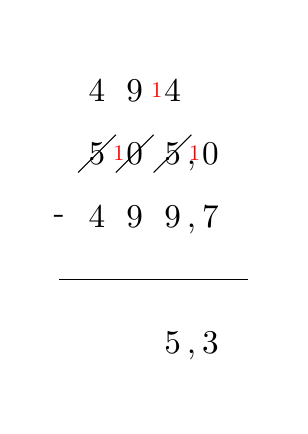
\begin{tikzpicture}[baseline,scale = 0.8]

    \tikzset{
      point/.style={
        thick,
        draw,
        cross out,
        inner sep=0pt,
        minimum width=5pt,
        minimum height=5pt,
      },
    }
    \clip (-0.5,0) rectangle (3.5,6);
    	\draw [color={black}] (2.4,4) node[anchor = center,scale=1.2, rotate = 0] {0};
	\draw [color={red}] (2.15,4) node[anchor = center,scale=0.8, rotate = 0] {1};
	\draw [color={black}] (2.4,3) node[anchor = center,scale=1.2, rotate = 0] {7};
	\draw [color={black}] (2.4,1) node[anchor = center,scale=1.2, rotate = 0] {3};
	\draw [color={black}] (1.8,4) node[anchor = center,scale=1.2, rotate = 0] {5};
	\draw[color ={black}] (1.4999999999999998,3.7)--(2.0999999999999996,4.3);
	\draw [color={black}] (1.8,5) node[anchor = center,scale=1.2, rotate = 0] {4};
	\draw [color={red}] (1.55,5) node[anchor = center,scale=0.8, rotate = 0] {1};
	\draw [color={black}] (1.8,3) node[anchor = center,scale=1.2, rotate = 0] {9};
	\draw [color={black}] (1.8,1) node[anchor = center,scale=1.2, rotate = 0] {5};
	\draw [color={black}] (1.2,4) node[anchor = center,scale=1.2, rotate = 0] {0};
	\draw[color ={black}] (0.8999999999999999,3.7)--(1.5,4.3);
	\draw [color={red}] (0.95,4) node[anchor = center,scale=0.8, rotate = 0] {1};
	\draw [color={black}] (1.2,5) node[anchor = center,scale=1.2, rotate = 0] {9};
	\draw [color={black}] (1.2,3) node[anchor = center,scale=1.2, rotate = 0] {9};
	\draw [color={black}] (0.6,4) node[anchor = center,scale=1.2, rotate = 0] {5};
	\draw[color ={black}] (0.3,3.7)--(0.8999999999999999,4.3);
	\draw [color={black}] (0.6,5) node[anchor = center,scale=1.2, rotate = 0] {4};
	\draw [color={black}] (0.6,3) node[anchor = center,scale=1.2, rotate = 0] {4};
	\draw [color={black}] (0,3) node[anchor = center,scale=1.2, rotate = 0] {-};
	\draw[color ={black}] (0,2)--(3,2);
	\draw [color={black}] (2.1,3.8) node[anchor = center,scale=1.2, rotate = 0] {,};
	\draw [color={black}] (2.1,2.8) node[anchor = center,scale=1.2, rotate = 0] {,};
	\draw [color={black}] (2.1,0.8) node[anchor = center,scale=1.2, rotate = 0] {,};

\end{tikzpicture}
\end{enumerate}

\end{EXO}

\begin{EXO}{}{}

 \opmul[lineheight=\baselineskip,columnwidth=2ex,displayshiftintermediary=all,decimalsepsymbol={,},voperator=bottom,voperation=top]{97.4}{9.8}\hspace*{30mm}\opmul[lineheight=\baselineskip,columnwidth=2ex,displayshiftintermediary=all,decimalsepsymbol={,},voperator=bottom,voperation=top]{9.8}{97.4}
\end{EXO}

\begin{EXO}{}{}

 \begin{tikzpicture}[baseline]

    \tikzset{
      point/.style={
        thick,
        draw,
        cross out,
        inner sep=0pt,
        minimum width=5pt,
        minimum height=5pt,
      },
    }
    \clip (-5,-4) rectangle (5,5);
    	\draw[color ={{black}},line width = 0.625,opacity = 0.8] (-1.0625,3.0625)--(-0.9375,2.9375);\draw[color ={{black}},line width = 0.625,opacity = 0.8] (-1.0625,2.9375)--(-0.9375,3.0625);
	\draw[color={black}] (-44.721359099991595,-22.360679549995798)--(48.721359099991595,24.360679549995798);\draw [color={black}] (0,0.5) node[anchor = center,scale=1, rotate = 0] {(d)};
	\draw[color={black}] (-1,3)--(0.4,0.2)--cycle;
	
	\draw [color={black}] (-1.22,3.45) node[anchor = center,scale=1, rotate = 0] {T};
	\draw [color={black}] (0.62,-0.25) node[anchor = center,scale=1, rotate = 0] {H};
	\draw [color={black}] (0.15,1.82) node[anchor = center,scale=1, rotate = -63.43495] {3,1 cm};
	\draw[color={black}] (0.22,0.56)--(0.58,0.74)--(0.76,0.38);

\end{tikzpicture}\\\\Pour mesurer la distance entre le point $T$ et la droite ($d$) :\\
      - on utilise l'équerre pour tracer la perpendiculaire à la droite ($d$)) qui passe par le point $T$\\
      - si on nomme $H$ le pied de la perpendiculaire, alors la distance entre le point $T$ et la droite ($d$) est la longueur $TH = 3{,}1 cm$
\end{EXO}

\begin{EXO}{}{}

\begin{enumerate}[itemsep=1em]
\item $7 \times 10$ s'écrit : {\bfseries \color[HTML]{f15929}le produit de 7 par 10}.
\item $14 \div 2$ s'écrit : {\bfseries \color[HTML]{f15929}le quotient de 14 par 2}.
\item $7+6$ s'écrit : {\bfseries \color[HTML]{f15929}la somme de 7 et de 6}.
\end{enumerate}

\end{EXO}

\clearpage
\end{Correction}
\end{document}

% Local Variables:
% TeX-engine: luatex
% End: